\chapter{Construção do painel}\label{cap_trabalho_academico}

Antes de avançar para a parte técnica, é importante explicar o que é o Centro de Inteligência da JFRN e como um painel poderia ajudar na tarefa deles. De acordo com o site do Centro de Inteligência, "O Centro de Inteligência da Justiça Federal do Rio Grande do Norte, criado pela Portaria nº 205/2017 – DF, em observância à Portaria nº 369/2017 – CJF, tem o objetivo de criar meios administrativos para prevenir demandas repetitivas, bem como de agilizar a sua tramitação processual, através do debate entre os seus componentes e os demais atores do sistema de justiça."

Esse tipo de demanda deve ser comunicado às autoridades para que a ação sobre esses processos repetitivos seja rápida, e não haja uma sobrecarga. Portanto, o painel será usado para auxiliar na análise dessas demandas, tentando acompanhar a evolução e desenvolvimento delas. Então, um painel que mostre os tipos de Assuntos mais recorrentes em cada Vara pode auxiliar o Centro de Inteligência a se preparar e comunicar embasado nos dados.

\section{Tecnologias usadas}

Uma das tarefas que fez parte do desenvolvimento do painel foi a pesquisa e escolha da ferramenta que poderia gerar a visualização, de forma rápida e com facilidade de ser distribuída pela infraestrutura de TI da JFRN. Como foi mostrado anteriormente, as ferramentas pagas custam caro, e a estrutura de desenvolvimento de painéis do TRF5 usa QlikView, que além de demandar uma licença para desenvolvimento, também precisa de alguns documentos para a publicação do painel. Então, algumas ferramentas gratuitas foram consideradas, e nesse processo de escolha foram analisados alguns pontos:

\begin{itemize}
	\item Pago ou gratuito: uma ferramenta paga pode exigir um custo alto para implementar e manter, então uma opção gratuita deve ser favorecida;
	\item Pronto ou próprio: existem softwares BI que já têm várias funções prontas, mas, nos casos do QlikView, PowerBI, Tableau, existem limitações que impedem a quantidade de linhas que serão lidas do conjunto de dados, por exemplo. Então, a criação das próprias análises e construção de gráficos foi o caminho escolhido.
\end{itemize}

Python é uma linguagem de programação de alto nível e de aplicações gerais, portanto, nada tem a ver como uma ferramenta pronta de BI, não tem integração automática de dados, nem criação simples de gráficos e visualizações, porém é completamente gratuita e tem um ótimo suporte da própria comunidade de usuários. De acordo com o \textit{TIOBE index}, que é um índice de popularidade de linguagens de programação, a linguagem Python é a terceira mais popular, ficando atrás de Java e C, a lista completa pode ser acessada na página do \href{https://www.tiobe.com/tiobe-index/}{TIOBE}.

\begin{table}[h]
	\centering
	\begin{tabular}{cc}
	\textbf{Linguagem}	& \textbf{Popularidade}  \\
	C	    &  16.95\% \\
	Java	& 12.56\% \\
	\textbf{Python}	& \textbf{11.28\%} \\
	C++	& 6.94\% \\
	C\#	& 4.16\% \\
	Visual Basic & 3.97\% \\
	JavaScript	& 2.14\% \\
	PHP	& 2.09\% \\
	R	& 1.99\% \\
	SQL	& 1.57\%
	\end{tabular}
	\caption{Linguagens de programação mais populares}
	\label{tab:my-table-2}
\end{table}

Para desenvolver o trabalho as bibliotecas Pandas, Plotly e Dash foram usadas, elas servem para analisar dados, gerar visualizações e montar o painel, respectivamente. Além do Python para construir o painel em si, foi usado o QlikView para extrair os dados e gerar um arquivo que pudesse ser lido pelo Pandas. Portanto, de forma resumida temos:

\begin{itemize}
	\item Python
	\begin{itemize}
		\item Dash
		\item Plotly
		\item Pandas
	\end{itemize}
	\item QlikView
\end{itemize}

\subsection{Justificando o Python}

Construir um painel usando Python pode apresentar alguns desafios, os desenvolvedores precisam ter noções de visualização de dados, análise de dados e programação com a linguagem. Mas, como foi dito anteriormente, a linguagem Python é bastante popular e não é difícil encontrar profissionais com esse perfil.

Outro ponto positivo de se usar Python é a replicabilidade, é possível criar painéis que atendam diversas Varas da JFRN, usando dados diferentes e gerando visualizações focadas na Vara. Essa forma de se desenvolver painéis mais simples não precisa ficar restrita ao Centro de Inteligência, ela pode expandir para atender necessidades mais simples, que não precisem do QlikView, de forma mais rápida mas atendendo às necessidades do gestor, levando em conta as características locais dos dados de onde for aplicado. 

É claro que esse tipo de expansão da TI deve ser acompanhada de um time maior de profissionais, com diferentes habilidades e competências, treinamentos relacionados a Python, visualização de dados, análises de dados etc. Mas os impactos disso seriam bons, os gestores teriam melhor controle sobre seus ambientes de trabalho, com novas visualizações e dados para basear novas estratégias por exemplo.


\section{Estrutura básica do painel}

Os dados usados são de uma análise feita para o Ministério Público Federal (MPF), essa análise já apresentava a divisão dos processos por Assunto e Vara, distribuídos ao longo dos meses. A partir dos dados, as visualizações começaram a ser feitas, usando Plotly, para tentar enxergar algum comportamento que pudesse ser útil aos gestores. Após isso, as visualizações foram embarcadas no Dash, e a estrutura mínima do painel ficou da seguinte forma:

\begin{figure}[h]
	\centering
	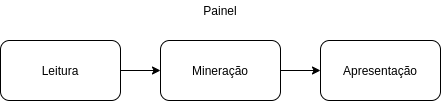
\includegraphics[scale=0.65]{./figures/cap2/estrutura_painel.png}
	\caption{Estrutura básica do painel}
\end{figure}

A leitura e mineração dos dados é feita pelo Pandas, e a apresentação pelo Dash. 

O painel que se propôs ao Centro de Inteligência não tem a estrutura clássica com diferentes tabelas (fato e dimensão), com as quais se geram as visualizações, no lugar disso, existe um arquivo .csv que contém os dados que serão usados, esses dados .csv fazem parte uma extração que veio do Processo Judicial eletrônico (PJe), e a partir desse arquivo o painel vai criar subconjuntos de acordo com o ano e órgão julgador escolhidos pelo usuário. Portanto, esse painel se aproxima mais de um visualizador de dados do que de um painel BI. Nele é possível selecionar duas variáveis: o Órgão Julgador e o Ano. A partir dessas escolhas o sistema vai fatiar os dados recebidos e mostrará algumas análises. Essas análises são mostradas em forma de tabelas condicionais, que mudam as cores das células de acordo com a frequência de aparição dos Assuntos.

\subsection{Plotly e Dash}

A Plotly é uma empresa canadense que desenvolve ferramentas para análise e visualização de dados. Os serviços essenciais são gratuitos, basta carregar a biblioteca no programa e começar a usar, isso vale para o \textit{plotly graph objects} por exemplo, que gera gráficos interativos, e também vale para o Dash, que é um dos seus principais produtos. 

Plotly além de ser o nome da empresa, também é o nome da ferramenta de visualização de dados. Ela foi usada nas primeiras versões do painel, mas como a visualização passou a se concentrar nas tabelas, acabou saindo da versão atual.

A biblioteca Dash é um \textit{framework} usado para construir aplicações web que apresentem um visual simples de se configurar e que sirva para análises de dados, não é necessário (porém ajuda bastante) conhecer \textit{html} ou outras tecnologias de \textit{front-end} para montar um painel. O resultado pode ser distribuído pela internet, usando serviços como o \textit{Heroku}, de forma gratuita.

\subsection{Pandas}

O Pandas é essencial na execução do painel, ele carrega as ferramentas necessárias para a manipulação dos dados, como a seleção correta do Órgão Julgador escolhido, e o ano a ser visualizado. Além disso, ele também é responsável por montar os \textit{dataframes}, que são estruturas de dados, que servem de base para as tabelas e as avaliações por cores que é mostrada na visualização final.

\subsection{Estrutura dos dados}

Nessa primeira versão do painel os dados virão de um arquivo .csv gerado a partir do Qlikview, que é o software de BI padrão da JF. Esse arquivo carrega várias colunas, entre elas podemos citar número do processo, status, classe judicial, documento da parte, data do trânsito em julgado. Porém, para fazer a análise dos dados serão usadas as seguintes colunas:

\begin{itemize}
	\item Órgão Julgador - os órgão julgadores são as Varas da JFRN que ficam espalhadas pelo Estado, o usuário precisa selecionar um desses órgãos para visualizar os dados.
	
	\item Data Primeira Distribuição - essa é a data em que o processo chega na JFRN, mesmo que caia numa Vara que não seja da competência dele essa data é importante para analisar que Vara o recebeu e quando ele chegou na JFRN.
	
	\item Assunto - é o tema do processo, existem diferentes categorias em que um processo pode ser categorizado, e a partir desse campo é possível contar quantos processos de cada tipo deram entrada na JFRN.
	
	\item Assunto Código - diferentes assuntos possuem diferentes códigos, e a contagem dos processos se dá usando esse campo, que agrupa os códigos que são iguais e conta o total para saber quantos deram entrada na JFRN.
\end{itemize} 

A partir da escolha do Ano e Órgão Julgador, o painel irá fazer as análises e seleções relevantes, populando a tabela e mostrando ao usuário quais são os processos mais frequentes de cada mês, no Ano e Vara escolhidos.

\subsection{Análise de anomalias}

A detecção de anomalias é, uma conjunto de técnica que servem para identificar comportamentos que fogem do que é esperado. Um dos desafios do trabalho foi encontrar uma forma de se detectar os Assuntos que possuíssem alta frequência de entrada na JFRN, porque, teoricamente, cada Ano e cada Vara possuem diferentes distribuições de Assuntos, e um modelo de detecção de anomalia que se encaixa bem em um determinado período, pode não se encaixar em outros. São 15 órgãos julgadores diferentes, e os anos que podem ser consultados são de 2014 até 2020, então são 90 distribuições diferentes. Apesar disso, usamos uma abordagem simples mas eficaz.

Primeiro, há uma análise da média ($\overline{x}$) de Assuntos que entraram na Vara, essa análise leva em conta o ano selecionado e o ano anterior, após isso, o desvio padrão ($\sigma$) é calculado e novas variáveis são geradas.

As variáveis são:
\begin{itemize}
	\item $anom_2$ definida como: $$anom_2 = media_{assuntos} + (2*\sigma)$$
	
	\item $anom_1$ definida como: $$anom_1 = media_{assuntos} + \sigma$$
	
	\item $media_{assuntos}$ que é a média simples dos assuntos, a cada dois anos:
	$$media_{assuntos} = \sum\limits_{ano}^{ano-1}\frac{assuntos}{total_{meses}}$$
\end{itemize}

Com essas variáveis encontradas, a distribuição das cores segue as regras a seguir, em que $total$ significa a quantidade total de Assuntos de determinada categoria:

\begin{equation}
	F_{cores} =
	\begin{cases}
		Vermelho & \text{se $total \geq anom_2$}\\
		Amarelo & \text{se $total \geq anom_1 \;e\; total < anom_2$}\\
		Verde & \text{se $total \geq media_{assuntos} \;e\; total < anom_1$}
	\end{cases}       
\end{equation}

Dessa forma é possível ver quais são os Assuntos que estão entrando com alta frequência, essa visualização deve ser usada para justificar uma possível análise, feita pelo gestor, para entender se essa frequência é realmente uma anomalia, ou se isso era esperado.

Ao longo do tempo o painel sofreu diversas mudanças. Essas mudanças foram incrementais e uma das principais fontes de exemplos e usos das ferramentas do Dash foi a plataforma Medium, que apresenta vários artigos exemplificando formas de se usar o Dash e como usar melhor os recursos da biblioteca. Um desses artigos do Medium foi muito importante para a definição de uma estrutura base de desenvolvimento do painel, o texto de Ishan Mehta \cite{medium1} apresenta uma proposta de estrutura que pode ser replicada e melhorada em trabalhos futuros, e a partir dessa estrutura o painel foi montado e desenvolvido, com novas visualizações e diferentes análises.

Na figura abaixo é possível ver um exemplo da aplicação das fórmulas no painel.
\begin{figure}[h]
	\centering
	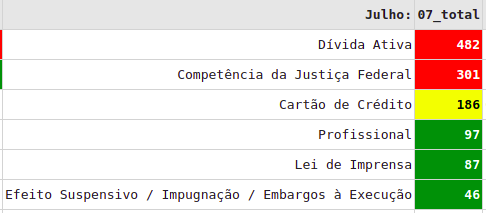
\includegraphics[scale=0.65]{./figures/cap2/exemplo_painel.png}
	\caption{Tabela com as diferentes frequências de Assuntos}
\end{figure}
